\documentclass[12pt]{article}
\usepackage[utf8]{inputenc}
\usepackage{geometry}
\usepackage{multicol}
\usepackage{listings}
\usepackage{color}
\usepackage{graphicx}
\usepackage{mathrsfs}
\usepackage{amsmath,amssymb,amsthm,enumitem}
\usepackage[makeroom]{cancel}
\geometry{margin=2cm}

\usepackage{xcolor}

\usepackage{styles/style}

%size 8.5 x 11 in
\title{Pruebas}
\author{rafael.rvp98 }
\date{September 2018}

\begin{document}
%\maketitle

\newgeometry{margin = 0in}
%Barra Azul
\hspace*{-0.9cm}
\vspace{-3mm}
\colorbox{azul2}{\makebox[8.5in][r]{\shortstack[r]{\vspace{2.75in}}}}

%Barra Blanca
\hspace*{-0.9cm}
\colorbox{blanco}{\makebox[8.5in][r]{\vspace{1mm}}}\\

\hspace*{-0.9cm}
%\setlength{\fboxsep}{5pt}
\colorbox{white}{\makebox[8.25in][l]{\hfill\shortstack[r]{\fontsize{36}{36}\rmfamily\color{azul1}Introducción a Machine Learning \&\\
\fontsize{36}{36}\rmfamily\color{azul1}Data Science}}}

\hspace*{-0.9cm}
\colorbox{blanco}{\makebox[8.5in][r]{\vspace{0.02mm}}}\\

%Barra Azul

%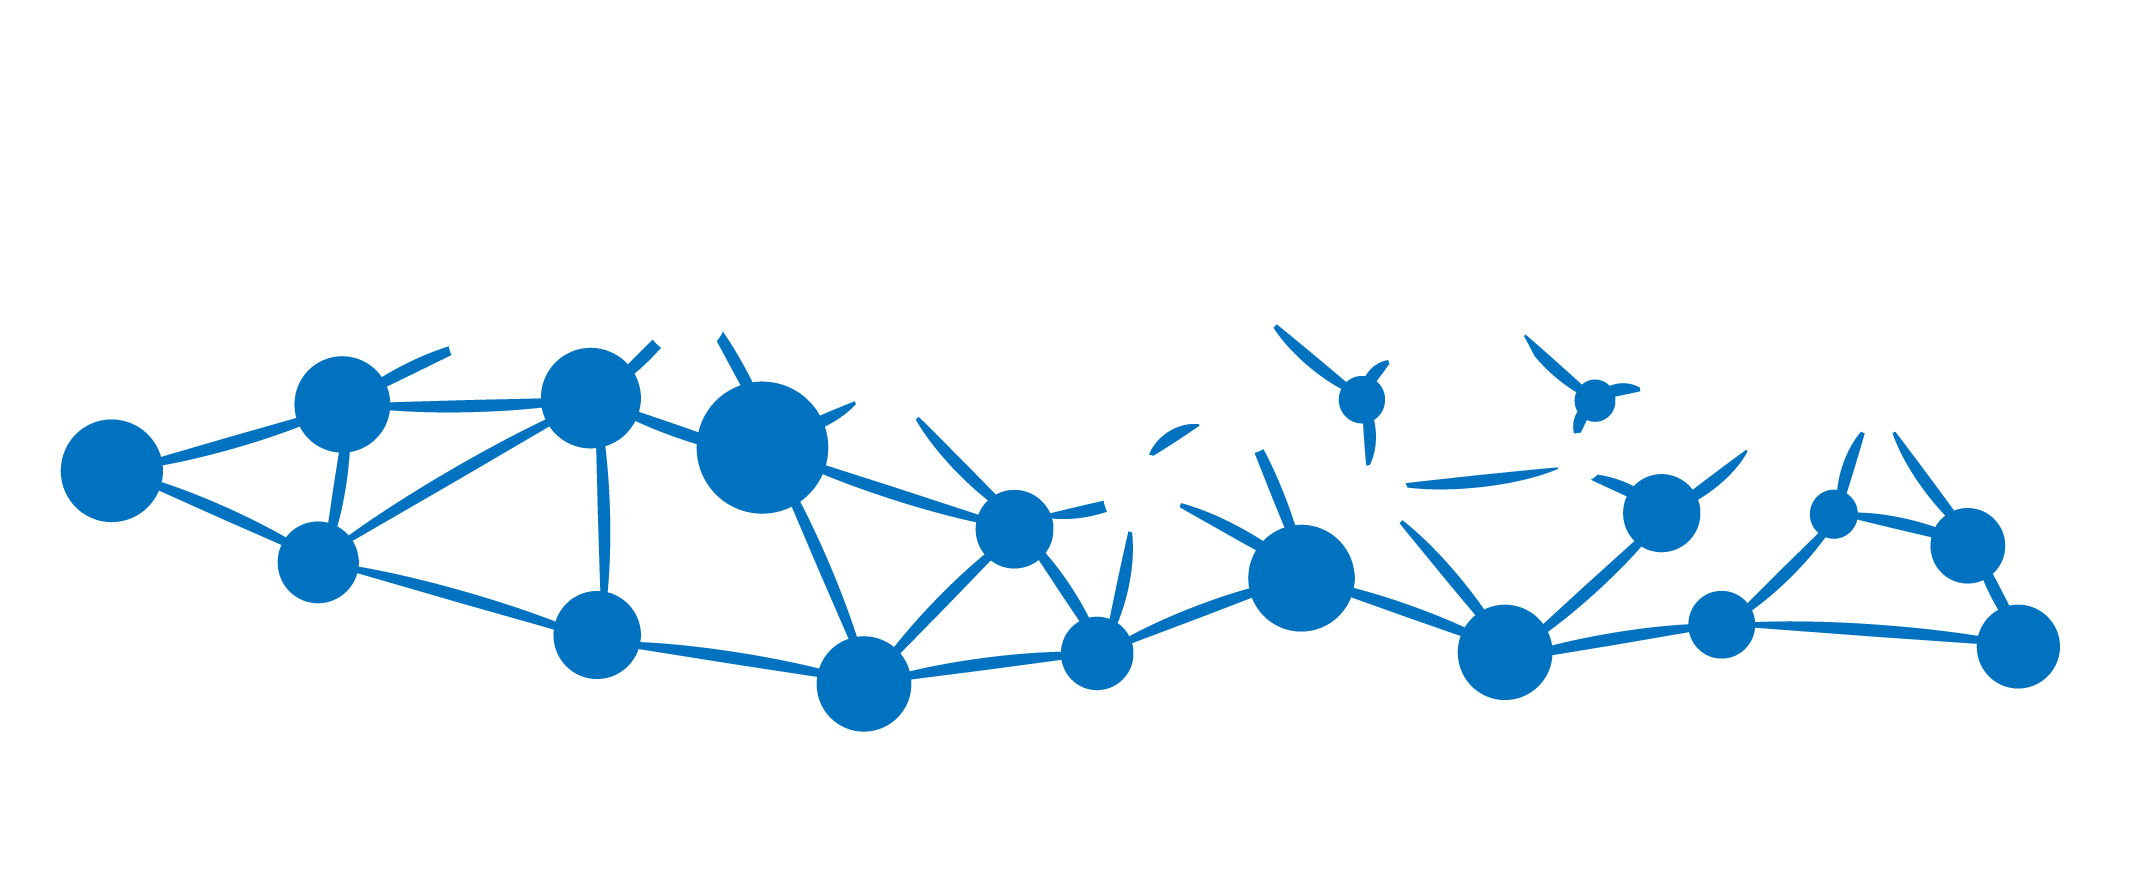
\includegraphics[width=3.09in]{images/transparente-tiny.png}
\vspace{-4.5mm}
\hspace*{-0.9cm}
\colorbox{azul2}{\makebox[8.5in][r]{\shortstack[r]{\vspace{5.8in}}}}

%logo
\vspace{-3mm}
\hspace*{-0.9cm}
\colorbox{azul2}{\makebox[8.5in][r]{\shortstack[r]{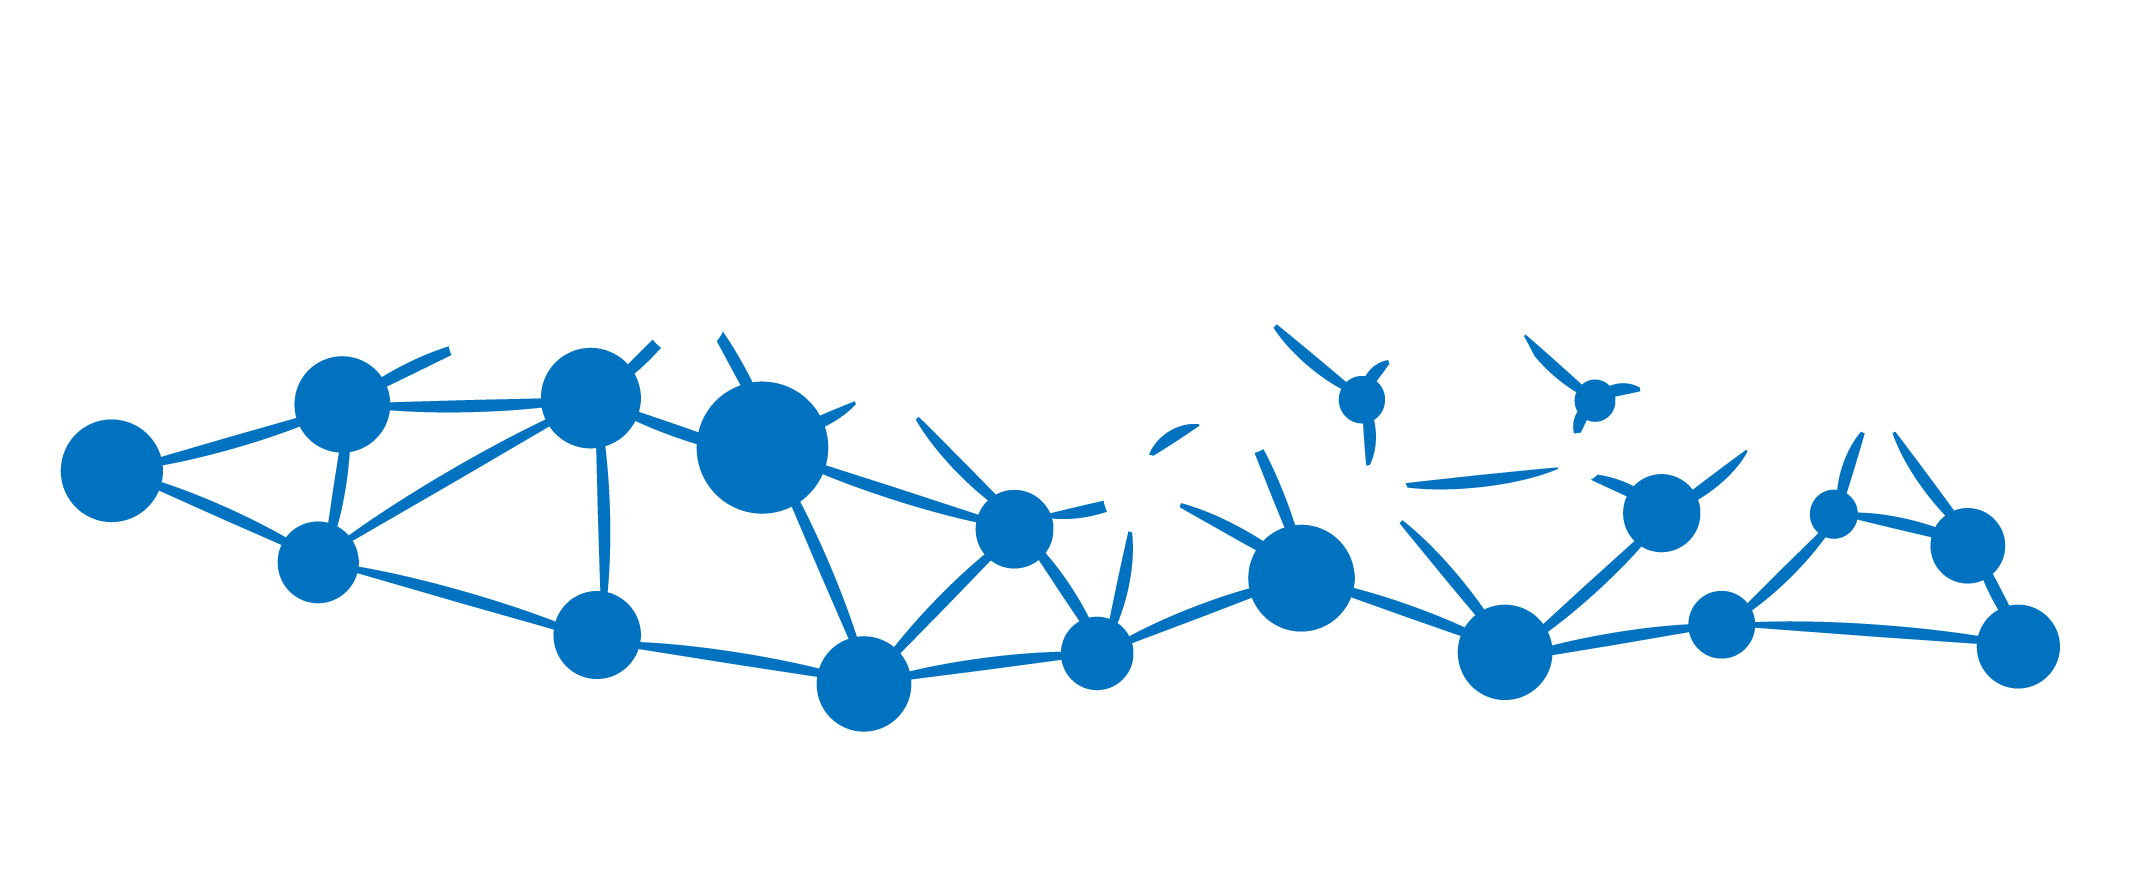
\includegraphics[scale=0.08]{images/transparente-tiny.png}}}}

\restoregeometry

\newpage
\section*{\fontsize{25}{25}\rmfamily\color{celeste}1. Plan de Avance}
\vspace*{1.5cm}
\fontsize{15}{15}\rmfamily\color{celeste}
\begin{enumerate}
	\item \textbf{Modelos Clásicos}
	\begin{itemize}
		\item Python para Machine Learning y Ciencia de Datos
		\item Métodos no Estadísticos
		\begin{itemize}
			\item K Vecinos más Cercanos
			\item Árboles de Decisión y Random Forest
		\end{itemize}
		\item Regresión Lineal y Métodos de Selección de Variables
		\item Regresión Logística
		\item \textbf{Proyecto de Medio Avance}
	\end{itemize}
	
	\item \textbf{Modelos Avanzados y Análisis de Datos}
	\begin{itemize}
		\item La Red Neuronal
		\item Reducción de Dimensionalidad
		\begin{itemize}
			\item PCA
			\item TSNE
		\end{itemize}
		\item Clustering
		\begin{itemize}
			\item K Means
			\item DBSCAN
			\item Gaussian Mixture
		\end{itemize}
		\item \textbf{Proyecto Final}
	\end{itemize}
\end{enumerate}

\newpage
\newgeometry{margin=0in}
%\colorbox{azul1}{\makebox[3.22in][r]{\shortstack[r]{\vspace{3in}}}}

%\vspace{-5mm}
\hspace*{-0.9cm}
\colorbox{white}{%
	\shortstack[r]{
		\makebox[5.2in][r]{\shortstack[r]{\vspace{3in}}}\\
		\parbox{5in}{%
			\begin{enumerate}
				\item Hello
				\item world!
			\end{enumerate}%
		}%
		\\
		\makebox[5.2in][r]{\shortstack[r]{\vspace{3in}}}
	}
	%\colorbox{gris}{\makebox[3.22in][r]{\shortstack[r]{\vspace{9in}}}}
}
\hspace*{-2mm}
\hfill \colorbox{gris}{\makebox[3.22in][r]{\shortstack[r]{\vspace{9in}}}}

\newpage

\hspace*{1cm}
\colorbox{white}{%
	\shortstack[r]{
		\makebox[5.4in][r]{\shortstack[r]{\vspace{1.98in}}}\\
		\parbox{5.4in}{%
			\section*{\fontsize{25}{25}\rmfamily\color{celeste}1. Plan de Avance}
			\vspace*{1.5cm}
			\fontsize{15}{15}\rmfamily\color{celeste}
			\begin{enumerate}
				\item \textbf{Modelos Clásicos}
				\begin{itemize}%
					\item Python para Machine Learning y Ciencia de Datos
					\item Métodos no Estadísticos
					\begin{itemize}%
						\item K Vecinos más Cercanos
						\item Árboles de Decisión y Random Forest
					\end{itemize}%
					\item Regresión Lineal y Métodos de Selección de Variables
					\item Regresión Logística
					\item \textbf{Proyecto de Medio Avance}
				\end{itemize}%
				\item \textbf{Modelos Avanzados y Análisis de Datos}
				\begin{itemize}%
					\item La Red Neuronal
					\item Reducción de Dimensionalidad
					\begin{itemize}%
						\item PCA
						\item TSNE
					\end{itemize}%
					\item Clustering
					\begin{itemize}%
						\item K Means
						\item DBSCAN
						\item Gaussian Mixture
					\end{itemize}%
					\item \textbf{Proyecto Final}
				\end{itemize}%
			\end{enumerate}%
		}%
		\\
		\makebox[5.2in][r]{\shortstack[r]{\vspace{3in}}}
	}
}
\hspace*{-2mm}
\hfill \colorbox{gris}{\makebox[2.2in][r]{\shortstack[r]{\vspace{11.61in}}}}


\end{document}
